\subsection{Insights into Digital Twin Technology in Industry 4.0}

% Adoption, Security Services, and Enabling Technologies}
% We provide estimation for distribution of reference points based on percent
% Blockchain is mostly used to provide some sort of security and privacy for data sharing and exchange in digital twin ecosystem. However, for one scenario which is detection, blockchain is leverage to provide detection.
% Machine learning mostly used in power grid for anomaly and intrusion detection 
% cloud computing is the enabling technology that we have observed in various sectors and for different kind of purpose including detectin, access control, testing, security management. 
% Testing includes performing vulnerability assessment and penetration testing. It is the most widly used of Digital Twin. This is becuase Digital Twin is grete for performing testing without distribution the ongoing operation of business. 

% How we make the analysis for sector 
% we include 


% predictive analytics, security management are not included for the analysis 

As part of a systematic literature review, this analysis focuses on the use of Digital Twin technology in Industry 4.0. We explore the enabling technologies used, the adoption of Digital Twin across different sectors, and the security services provided by Digital Twin. By examining these aspects, this analysis aims to provide insight into the current landscape of Digital Twin in terms of key technologies used, industry sectors targeted, and security functionalities associated with this technology. 

\subsubsection*{Digital Twin Adoption by Sector}
Fig \ref{fig:sector} provides insights into the adoption of digital twins based on their use cases or targeted industry sectors. The data are the result of data extraction from the reviewed papers. The CPS/ICS (Cyber-Physical Systems/Industrial Control Systems) sector emerges as the main area for digital twin adoption. It is worth noting that, CPS/ICs is an umbrella term that includes other specific industries like smart cities, oil and gas, etc. 

When it comes to specific industries, the power grid sector stands out as the most extensively researched area for the deployment of digital twins. It is observed that Digital Twin technology is primarily utilized in this sector to enable anomaly detection. It is worth noting that other services such as vulnerability assessment, access control, simulation, security management, and situational awareness have also been explored. The automotive and intelligent transport sectors also widely adopted Digital Twin to protect and secure vehicles, transportation systems, and traffic management. Other sectors, such as 5G network, aerospace, agriculture, satellite, enterprise network, and water, show smaller but notable percentages, reflecting the diverse range of industries using Digital Twin technology. 

\begin{figure}[H]    
    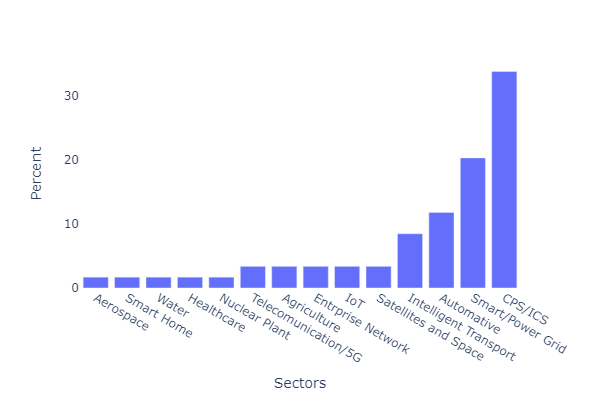
\includegraphics[width=1\textwidth]{images/rt/dt-sector.png}
    \caption{Use Case of Digital Twin}
    \label{fig:sector}
\end{figure}


% \begin{tikzpicture}
% \begin{axis}[
% 	x tick label style={
% 		/pgf/number format/1000 sep=},
% 	ylabel=Year,
% 	enlargelimits=0.05,
% 	legend style={at={(0.5,-0.1)},
% 	anchor=north,legend columns=-1},
% 	ybar interval=0.7,
% ]
% \addplot 
% 	coordinates {(2012,408184) (2011,408348)
% 		 (2010,414870) (2009,412156)};
% \addplot 
% 	coordinates {(2012,388950) (2011,393007) 
% 		(2010,398449) (2009,395972)};
% \legend{Men,Women}
% \end{axis}
% \end{tikzpicture}


\subsubsection*{Digital Twin as Security Tool}

The first research question (\textbf{RQ1)}) of this paper seeks to explore the utilization of Digital Twin as a security tool. Indeed, Digital Twin proves to be an integrated platform capable of delivering a wide range of security services, as evidenced by the papers reviewed in this work. Given its nature as an exact replica of assets and processes, Digital Twin can be used to provide security-related operations without causing any disruptions to the actual ongoing processes.

Hence, Digital Twin as a security tool can provide a simulation environment to enhance security skills (cyber range), predictive analytics capability in terms of forecasting attacks and security weaknesses, a testing environment for conducting vulnerability assessment penetration testing, anomaly and intrusion detection by processing data generated from the Digital Twin and actual environment and an environment for access control. 

In addition, a limited number of papers highlighted Digital Twin can be used to provide functionality such as data visualization, threat modelling, situational awareness and data sharing, all of which can be leveraged for security purposes. 


\begin{figure}[H]    
    {
        \centering
        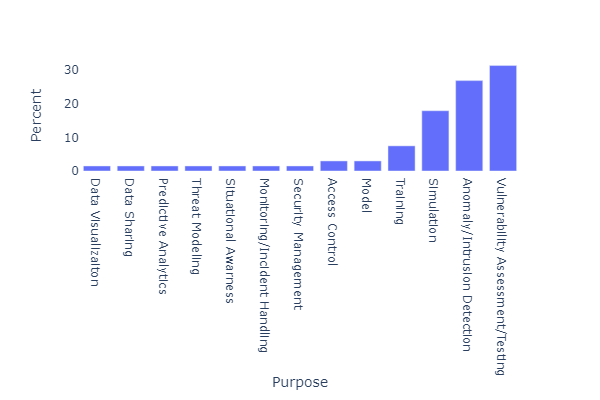
\includegraphics[width=1\textwidth]{images/rt/dt-securityservice.png}
        \caption{Distribution of Papers Based on Security Service Provided By Digital Twin.}
        \label{fig:use}
    }
\end{figure}

Fig \ref{fig:use} focuses on security services provided by Digital Twin technology within various industries. Testing, encompassing activities such as vulnerability assessment and penetration testing, emerges as the most widely adopted practice. This is attributed to the inherent capability of Digital Twins to facilitate rigorous testing procedures without disrupting the ongoing operations of a business.  Anomaly and Intrusion detection is the next most prominent security service provided. Specifically, in the power grid and smart grid sector, it is the primary motivation behind the deployment of the Digital Twin.


\subsubsection*{Enabling Technologies Integrated With Digital Twin }

Based on the literature review, the most prominent technologies that power Digital Twins are AI, Blockchain, Cloud and Edge Computing, Analytics and Big-data. AI is an umbrella term to represent various technologies including ML, Deep learning (DL). In general, machine learning encompasses analytical operations; however, analytics, by itself, lacks the inherent learning capability exhibited by machine learning. In other words, analytics is a "Data Science" field for collecting and representing data to identify patterns and insight \cite{fuller_digital_2020}. On the other hand, Big-data technology is used to store and process large-scale data. 

To avoid bias, we categorize the papers when any of the enabling technologies are explicitly mentioned as being used within the Digital Twin to augment its capabilities.  

\begin{figure}[H]  
    {
        \centering
        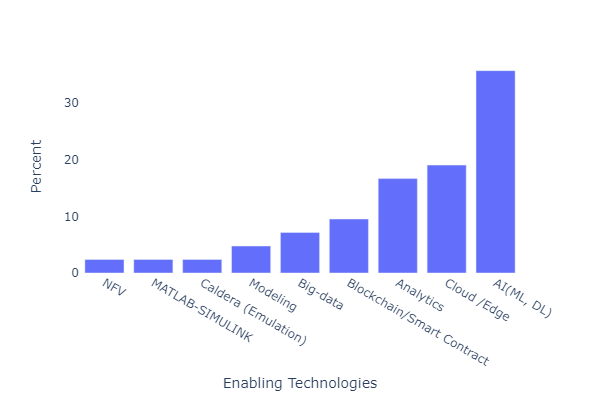
\includegraphics[width=1\textwidth]{images/rt/dt-enablingtech.png}
        \caption{Distribution of Papers Based on Enabling Technology Integrated With Digital TWin}
        \label{fig:enable}
    }
\end{figure}

Fig \ref{fig:enable} (C) shows the distribution of enabling technologies used or implemented with digital twin technology to provide various functionalities and services. Among the enabling technologies, machine learning (ML) emerges as the most dominant Digital Twin functionality augmenter. Different ML algorithms and models were proposed in the literature to equip Digital Twin with the capability of data analysis, predictive insight, anomaly, and intrusion detection. Cloud computing along with edge computing plays a key role in supporting the storage, and processing of large amounts of data. Additionally, blockchain technology is used with Digital Twin mainly to enhance the security and privacy of shared data.


\subsection{Security Mechanisms Analysis From Literature}
Securing the communication channel between Digital Twin and (I)IoT deployment is a critical concept that should not be neglected especially in the critical infrastructure of Industry 4.0. To address this, a few research efforts on various security mechanisms are presented in the literature. In this subsection, a comparative analysis of security mechanisms for secure data communication in terms of resource efficiency and deployment practicality is presented. 

The most widely used approach to provide privacy and security in the Digital Twin ecosystem in the existing literature is Blockchain (Smart Contract) technology. In \cite{kumarBlockchainDeepLearning2022, salimBlockchainEnabledSecureDigital2022, zhengBlockchainBasedTrustworthy2022a, liuBlockchainBasedSecureCommunication2022a, danilczykBlockchainChecksumEstablishing2021a, chenDigitalTwinBasedHeuristic2023a} Blockchain-based data transmission scheme for data integrity are proposed. Due to the inherent nature of Blockchain, the proposed solution based on this technology have a limitation in providing data confidentiality. Blockchain-based security approaches offer data integrity in a distributed environment but they may have computationally demanding underlying technology, impacting their suitability for resource-constrained IoT devices.

Three studies \cite{xuEfficientAuthenticationVehicular2021, wuDeepLearningDriven2022, chengzhelaiSPDTSecurePrivacyPreserving2022, pervezSIGNEDSmartCIty2023a} focused on providing privacy using techniques such as secret-handshake scheme, group signature and differential privacy techniques. While enhancing privacy, these two approaches may require significant computational resources for cryptographic operations on resource-constrained (I)IoT devices.

Furthermore, we encounter security mechanisms that focus on access control and trust \cite{gehrmannDigitalTwinBased2020, chengzhelaiSPDTSecurePrivacyPreserving2022, debenedictisAdoptionSecureCyber2022}. the first paper suggest a centralized access control system using XACML policies and tokens like SAML and OAuth to regulate access and ensure communication security. In another paper, the authors proposed a scheme for secure data sharing using attribute-based access control, in the thrid paper the authors propose secure data exchange between Digital Twin and (I)IoT using technologies namely PUF (Physical Unclonable Functions) and TPM (Trusted Platform Module ). Though these solutions are resource efficient, they may not be economically practical to use them as the special hardware setup and complex key management involved. 


Lastly, we explore a unique study \cite{lvDigitalTwinsBased2022} based on quantum communication and quantum entanglement. It is a theoretical proposed solution that may not even be possible in the near future as this technology has not yet developed. Therefore, quantum communication might provide very efficient and strong security but it might also require sophisticated hardware, that will make it challenging to implement it practically. 



